\chapter{Payload Deployment}

During the boost, coast, and the majority of the launch vehicle's flight, the payload will remain idle and securely fixed in the payload bay. This chapter will detail the means of securement and deployment of the payload, as well as a trade-off between the various means that have been consider to arrive at the leading design.

This chapter will be structured as follows: Sec.~\ref{PL:Deployment:Requirements} details the requirements the payload is to satisfy given the overall mission and top-level requirements, followed by a trade-off study regarding the means of securement in Sec.~\ref{PL:Deployment:Securement}, as well as the possible deployment modes in Sec.~\ref{PL:Deployment:Deployment}. Finally, the leading design is presented in Sec.~\ref{PL:Deployment:LeadingDesign} in reference to the foregoing trade-off studies.


\section{Requirements}\label{PL:Deployment:Requirements}

This section details the various requirements to which the payload deployment scheme must abide. Specifically, two forms of requirements are identified: top-level requirements and team-derived requirements. The first are requirements either imposed by the competition, or legislation that is in effect at the time of launch and operations. The second form of requirements pertain to what the team perceives to be of importance in assuring mission success and robustness.

\subsection{Top-level requirements}

The top-level requirements for the payload deployment are outlined in Secs. 4.3--4 of \citep{MSFC2019}, reading as follows:

\begin{enumerate}[noitemsep, label=4.\arabic*.]
	\setcounter{enumi}{3}
	\item Lunar Ice Sample Recovery Mission Requirements
	\begin{enumerate}[noitemsep, label=4.3.\arabic*.]
		\setcounter{enumi}{5}
		\item Teams must abide by all \gls{faa} and \gls{nar} rules and regulations.
		\item Black Powder and/or similar energetics are only permitted for deployment of in-flight recovery systems. Any ground deployments must utilize mechanical systems.
		\item Any part of the payload or vehicle that is designed to be deployed, whether on the ground or in the air, must be fully retained until it is deployed as designed.
		\begin{enumerate}[noitemsep, label=4.3.7.\arabic*.]
			\item A mechanical retention system will be designed to prohibit premature deployment.
			\item The retention system will be robust enough to successfully endure flight forces experienced during both typical and atypical flights.
			\item The designed system will be fail-safe.
			\item Exclusive use of shear pins will not meet this requirement.
		\end{enumerate}
	\end{enumerate}
	\item Special Requirements for UAVs and Jettisoned Payloads
	\begin{enumerate}[noitemsep, label=4.4.\arabic*.]
		\item Any experiment element that is jettisoned during the recovery phase will receive real-time \gls{rso} permission prior to initiating the jettison event.
		\item \gls{uav} payloads, if designed to be deployed during descent, will be tethered to the vehicle with a remotely controlled release mechanism until the \gls{rso} has given permission to release the UAV.
		\item Teams flying \acrshortpl{uav} will abide by all applicable \gls{faa} regulations, including the \gls{faa}'s Special Rule for Model Aircraft (Public Law 112-95 Section 336; see \url{https://www.faa.gov/uas/faqs}).
		\item Any \gls{uav} weighing more than .55 lbs. will be registered with the \gls{faa} and the registration number marked on the vehicle.
	\end{enumerate}
\end{enumerate}

In addition, by \gls{faa} regulations \citep{FederalAviationAdministration2018}, the \gls{uav} may only be operated below \SI{400}{\feet} in \gls{los}\footnote{FAA Reauthorization Act of 2018 \S 346(b.2.C), 49 U.S.C. \S 44806}. From the FAA Reauthorization Act of 2018, the following pertinent regulations may be found. The \gls{uav} must have a gross weight under \SI{4.4}{\poundm}, and must be operated:

\begin{enumerate}[noitemsep, label=(\roman*)]
	\item within or beyond visual \gls{los} of the operator;
	\item less than \SI{400}{\feet} above ground;
	\item during daylight conditions;
	\item within Class G airspace; and
	\item outside of 5 statute miles from any airport, heliport, seaplane base, spaceport, or other location with aviation activities.
\end{enumerate}

As a supplement to these regulations, an aeronautical chart of the surroundings of the launch site (Bragg Farms, Hazel Green, AL) is given in Fig.~\ref{fig:PL:Deployment:VFRchart}.

\begin{figure}[H]
	\centering
	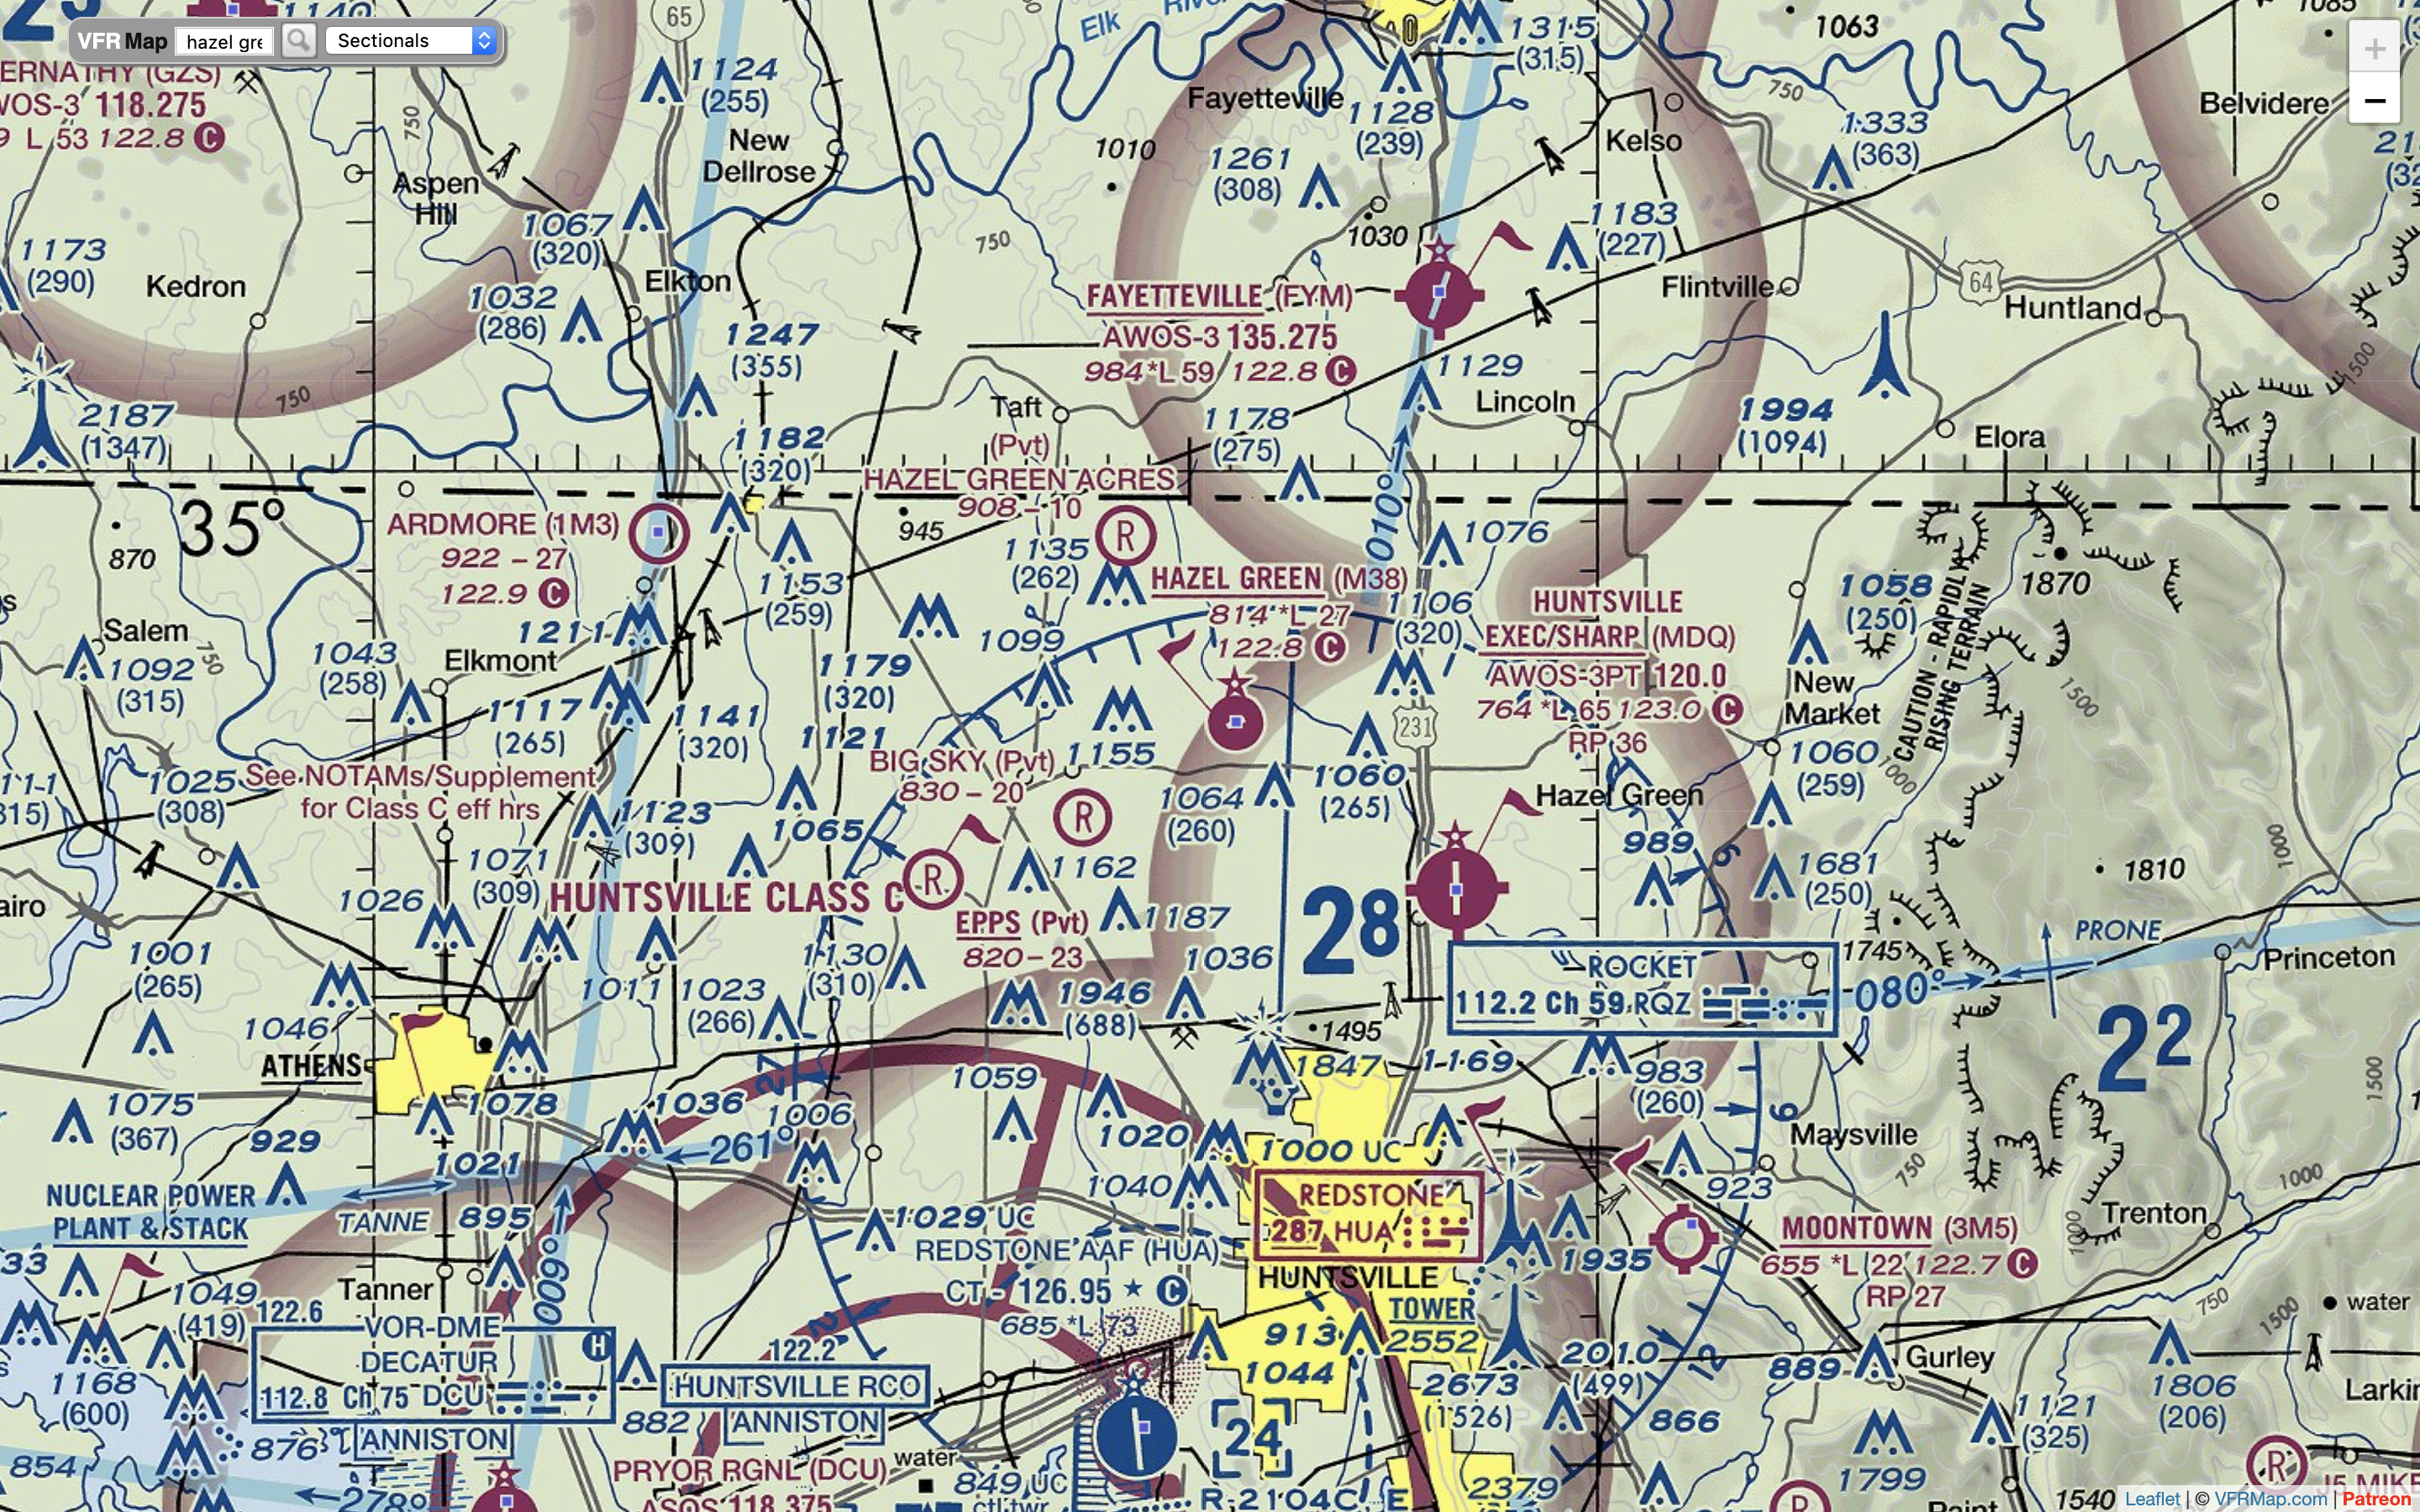
\includegraphics[width=0.75\linewidth]{img/PL/AeronauticalChart}
	\caption[VFR aeronautical chart of the Hazel Green, AL area]{\gls{vfr} aeronautical chart of the Hazel Green, AL area. Adapted from \href{http://vfrmap.com/}{VFRMap.com}}
	\label{fig:PL:Deployment:VFRchart}
\end{figure}

In this chart, the Class E airspace is bounded by a vignette magenta border, and spans down to \SI{700}{\feet}; anything below that is Class G airspace, and thus open for \gls{uav} operations. Incidentally, the area of payload operations lies beyond a 5 mile radius of the closest airfield.

\subsection{Team-derived requirements}

In addition to the above, a number of additional requirements have been compiled by the team. In particular, the robustness of the securement system, as well as the reliability of the deployment system are at the center of the discussion\todo[author=HE]{Draft team-derived requirements}.


\section{Means of Securement}\label{PL:Deployment:Securement}

\section{Means of Deployment}\label{PL:Deployment:Deployment}

\section{Leading Design}\label{PL:Deployment:LeadingDesign}